\documentclass[12pt,a4paper]{article}

% ── Encoding & Language ──────────────────────────────────────────────────────
\usepackage[utf8]{inputenc}
\usepackage[T1]{fontenc}

% ── Layout ───────────────────────────────────────────────────────────────────
\usepackage[top=2.5cm, bottom=2.5cm, left=3cm, right=2.5cm]{geometry}
\usepackage{setspace}
\onehalfspacing
\usepackage{indentfirst}
\setlength{\parindent}{1.25cm}
\setlength{\parskip}{0pt}

% ── Fonts & Typography ───────────────────────────────────────────────────────
\usepackage{lmodern}
\usepackage{microtype}

% ── Graphics & Tables ────────────────────────────────────────────────────────
\usepackage{graphicx}
\usepackage{booktabs}
\usepackage{caption}
\usepackage{subcaption}
\usepackage{float}
\usepackage{array}
\usepackage{xcolor}

% ── Math ─────────────────────────────────────────────────────────────────────
\usepackage{amsmath}

% ── Hyperlinks ───────────────────────────────────────────────────────────────
\usepackage[hidelinks]{hyperref}
\renewcommand{\contentsname}{Sumário}

% ── Headers & Footers ────────────────────────────────────────────────────────
\usepackage{fancyhdr}
\pagestyle{fancy}
\fancyhf{}
\fancyhead[L]{\small Laboratório de Experimentação de Software}
\fancyhead[R]{\small PUC Minas -- 2026/1}
\fancyfoot[C]{\thepage}
\setlength{\headheight}{14pt}
\renewcommand{\headrulewidth}{0.4pt}

% ─────────────────────────────────────────────────────────────────────────────
\begin{document}

% ── Capa ─────────────────────────────────────────────────────────────────────
\begin{titlepage}
  \centering
  \vspace*{2.0cm}

  {\normalsize
    Pontifícia Universidade Católica de Minas Gerais (PUC~Minas)\\
    Laboratório de Experimentação de Software -- 2026/1
  }

  \vspace*{2.8cm}

  {\large
    Raphael Brito\\[0.3em]
    Yan Cota
  }

  \vspace*{4.2cm}

  {\LARGE \textbf{Laboratório 01}\\[0.5em]
  \Large Características de Repositórios Populares do GitHub}

  \vfill

  {\normalsize Belo Horizonte\\ 2026}
\end{titlepage}

% ── Sumário ──────────────────────────────────────────────────────────────────
\pagenumbering{roman}
\tableofcontents
\newpage
\pagenumbering{arabic}
\setcounter{page}{1}

% ─────────────────────────────────────────────────────────────────────────────
\section{Introdução}
% ─────────────────────────────────────────────────────────────────────────────

O GitHub hospeda hoje mais de 300 milhões de repositórios públicos, tornando-se
a maior plataforma de desenvolvimento colaborativo do mundo. Neste trabalho
analisamos os \textbf{1000 repositórios mais populares} (medidos pelo número
de \textit{stars}) a fim de compreender suas características estruturais e de
processo de desenvolvimento.

Para isso, utilizamos a \textbf{API GraphQL do GitHub} para coletar dados como
data de criação, data de última atualização, linguagem primária, número de
\textit{pull requests} aceitas (merged), número de \textit{releases} e número de
\textit{issues} abertas e fechadas.

\section{Questões de Pesquisa e Hipóteses}

Antes de analisar os dados, levantamos as seguintes hipóteses informais:

\begin{description}
  \item[\textbf{H1 -- Maturidade}]
    Esperamos que repositórios populares sejam, em geral, \textbf{maduros},
    com pelo menos 3--5 anos de existência. A popularidade tende a se acumular
    com o tempo, à medida que mais usuários descobrem e marcam o projeto.

  \item[\textbf{H2 -- Contribuição externa}]
    Projetos populares devem atrair \textbf{muitas contribuições externas},
    resultando em um número elevado de PRs aceitas. Comunidades grandes são
    naturalmente mais ativas.

  \item[\textbf{H3 -- Frequência de releases}]
    Supomos que repositórios populares lancem releases com certa regularidade;
    entretanto, projetos de documentação/listas (como \textit{awesome-*})
    tipicamente \textbf{não utilizam releases}, o que deve fazer a mediana ser
    baixa.

  \item[\textbf{H4 -- Atualização recente}]
    Esperamos que a grande maioria dos repositórios populares esteja
    \textbf{atualizada recentemente} (últimos 30--60 dias), pois projetos
    abandonados raramente mantêm o topo do ranking.

  \item[\textbf{H5 -- Linguagens populares}]
    Acreditamos que linguagens como \textbf{JavaScript/TypeScript, Python e Java}
    dominem os repositórios populares, refletindo a popularidade dessas
    linguagens na comunidade open-source.

  \item[\textbf{H6 -- Alto percentual de issues fechadas}]
    Projetos ativos e com boa manutenção devem ter um \textbf{alto percentual
    de issues fechadas} (acima de 0,8), indicando equipes responsivas.

  \item[\textbf{H7 -- Linguagem e contribuição (Bônus)}]
    Esperamos que projetos escritos em linguagens mais populares
    (JavaScript, TypeScript, Python) recebam \textbf{mais contribuição externa},
    lancem mais releases e sejam atualizados com maior frequência.
\end{description}

% ─────────────────────────────────────────────────────────────────────────────
\section{Objetivos}
% ─────────────────────────────────────────────────────────────────────────────

\subsection{Objetivo Geral}

Caracterizar os 1000 repositórios mais populares do GitHub por meio de
métricas de produto e processo, avaliando maturidade, atividade, contribuição
externa, uso de releases, linguagem predominante e manutenção de issues.

\subsection{Objetivos Específicos}

\begin{itemize}
  \item Mensurar a idade dos repositórios e verificar evidências de maturidade.
  \item Quantificar contribuição externa por PRs aceitas.
  \item Avaliar a adoção de releases no ciclo de entrega.
  \item Medir a recência de atualização dos projetos.
  \item Identificar as linguagens mais frequentes entre os repositórios populares.
  \item Estimar a razão de issues fechadas como indicador de manutenção.
  \item Comparar PRs, releases e atualização entre linguagens (RQ07 bônus).
\end{itemize}

% ─────────────────────────────────────────────────────────────────────────────
\section{Metodologia}
% ─────────────────────────────────────────────────────────────────────────────

\subsection{Coleta de Dados}

A coleta foi realizada por meio da \textbf{API GraphQL do GitHub} em duas etapas:

\begin{enumerate}
  \item \textbf{Busca paginada de repositórios:} utilizamos a busca por
    \texttt{stars:>0 sort:stars-desc} com páginas de 100 repositórios,
    repetindo a paginação via \textit{cursor} até atingir os 1.000 repositórios
    mais estrelados.

  \item \textbf{Coleta de métricas:} para cada repositório coletamos, via
    consulta GraphQL em lotes de 4, o total de PRs aceitas
    (\texttt{pullRequests(states: MERGED)}\texttt{.totalCount}),
    o total de releases (\texttt{releases.totalCount}) e o total e
    número de issues fechadas.
\end{enumerate}

Os dados foram consolidados em um arquivo \texttt{repos.csv} com os seguintes
campos: \texttt{full\_name}, \texttt{stars}, \texttt{language},
\texttt{created\_at}, \texttt{updated\_at}, \texttt{age\_days},
\texttt{days\_since\_update}, \texttt{merged\_prs}, \texttt{releases},
\texttt{total\_issues}, \texttt{closed\_issues}, \texttt{closed\_issue\_ratio}.

\subsection{Análise}

Para cada questão de pesquisa utilizamos a \textbf{mediana} como medida de
tendência central, por ser robusta a valores extremos (outliers), comuns em
distribuições de métricas de software. Para variáveis categóricas (linguagem)
realizamos contagem por categoria. Os gráficos foram gerados com
\texttt{matplotlib} em Python.

\subsection{Visualização dos Dados}

As distribuições numéricas foram apresentadas por meio de histogramas
(RQs 01, 02, 03, 04 e 06). Para as RQs 02 e 03, utilizamos escala logarítmica
para reduzir o efeito de outliers. As análises por linguagem (RQ07) foram
representadas com boxplots, comparando medianas e dispersões por categoria.

% ─────────────────────────────────────────────────────────────────────────────
\section{Resultados}
% ─────────────────────────────────────────────────────────────────────────────

A Tabela~\ref{tab:summary} apresenta as medianas das métricas numéricas.
Para a RQ05 (variável categórica), a contagem por linguagem está na
Tabela~\ref{tab:rq05}.

\begin{table}[H]
  \centering
  \caption{Resumo das medianas das métricas (RQs 01, 02, 03, 04 e 06).}
  \label{tab:summary}
  \begin{tabular}{llr}
    \toprule
    \textbf{RQ} & \textbf{Métrica} & \textbf{Mediana} \\
    \midrule
    RQ01 & Idade (anos) & 8,39 \\
    RQ02 & PRs aceitas & 745 \\
    RQ03 & Releases & 40 \\
    RQ04 & Dias desde atualização & 0 \\
    RQ06 & Razão issues fechadas & 0,8676 \\
    \bottomrule
  \end{tabular}
\end{table}

% ─────────────────────────────────────────────────────────────────────────────
\subsection{Resultados por Questão de Pesquisa}
% ─────────────────────────────────────────────────────────────────────────────

% ──────────────────────────────────────────────────
\subsection{RQ01 -- Sistemas populares são maduros/antigos?}
% ──────────────────────────────────────────────────

\textbf{Métrica:} idade do repositório em anos (calculada a partir de
\texttt{created\_at}).

\textbf{Hipótese (H1):} repositórios populares tendem a ser maduros,
com 3--5 anos ou mais de existência.

\begin{figure}[H]
  \centering
  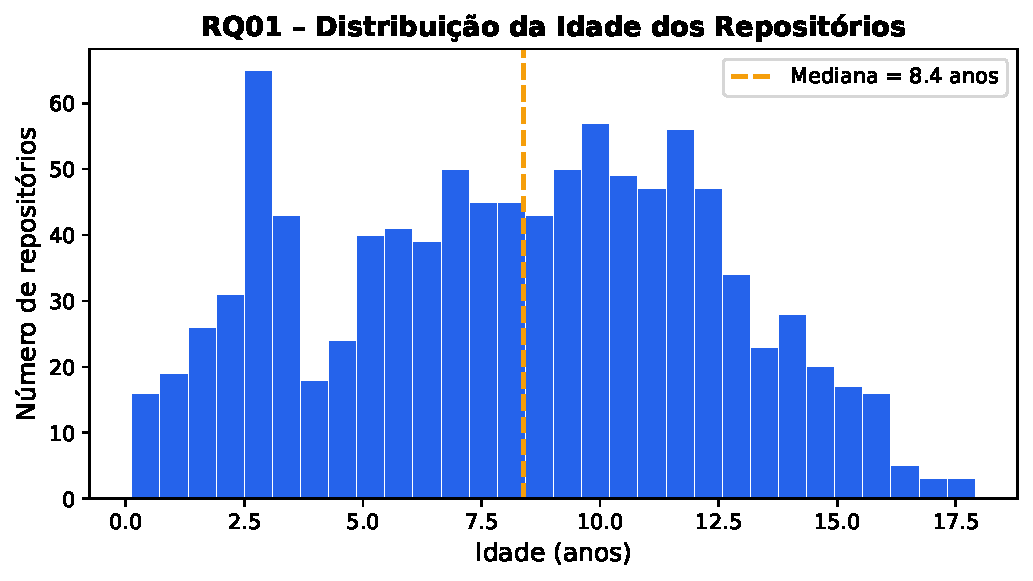
\includegraphics[width=0.85\textwidth]{figs/rq01_age.pdf}
  \caption{Distribuição da idade dos 1.000 repositórios mais populares.}
  \label{fig:rq01}
\end{figure}

\textbf{Resultado:} a mediana da idade é de \textbf{8,39 anos}
(3.062 dias). A distribuição é assimétrica à esquerda, com a maioria
dos repositórios concentrada entre 3 e 8 anos.

\textbf{Discussão:} a hipótese H1 foi \textbf{confirmada}. Repositórios populares
são, em geral, maduros. Há pouquíssimos repositórios populares com menos de
1 ano de existência, o que reforça que a popularidade se acumula com o tempo.

% ──────────────────────────────────────────────────
\subsection{RQ02 -- Sistemas populares recebem muita contribuição externa?}
% ──────────────────────────────────────────────────

\textbf{Métrica:} total de pull requests aceitas (\textit{merged}).

\textbf{Hipótese (H2):} projetos populares atraem muitas contribuições
externas e, portanto, apresentam alto volume de PRs aceitas.

\begin{figure}[H]
  \centering
  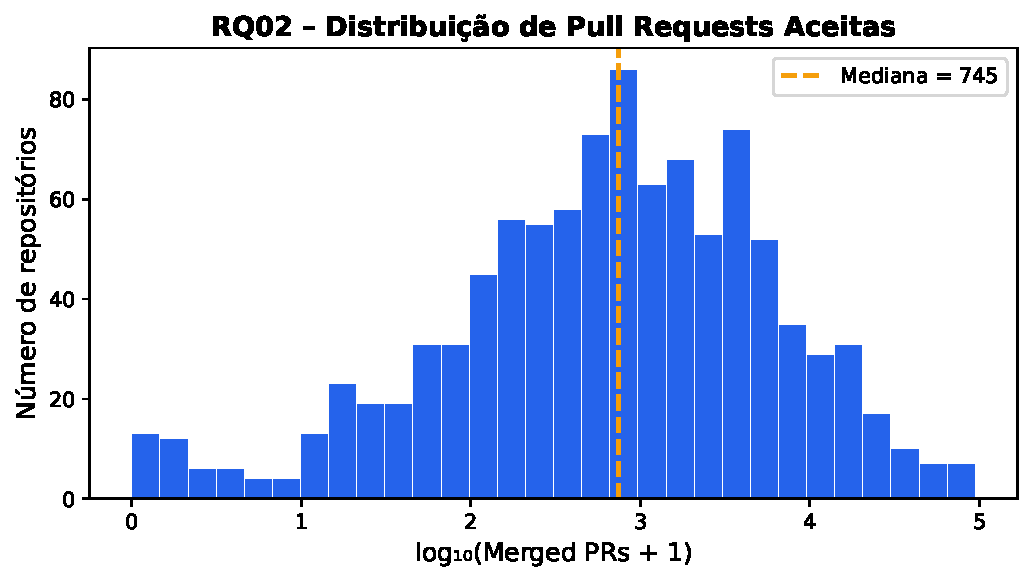
\includegraphics[width=0.85\textwidth]{figs/rq02_prs.pdf}
  \caption{Distribuição do número de PRs aceitas (escala log\textsubscript{10}).}
  \label{fig:rq02}
\end{figure}

\textbf{Resultado:} a mediana é de \textbf{745 PRs aceitas}.
A distribuição é bastante dispersa: projetos de documentação/listas apresentam
poucas PRs, enquanto projetos de código com grandes comunidades (e.g.,
\textit{VSCode}, \textit{TensorFlow}) chegam a dezenas de milhares.

\textbf{Discussão:} a hipótese H2 é \textbf{parcialmente confirmada}.
Embora a mediana é razoável, a grande variância indica que o volume de
contribuições externas depende fortemente do tipo de projeto.

% ──────────────────────────────────────────────────
\subsection{RQ03 -- Sistemas populares lançam releases com frequência?}
% ──────────────────────────────────────────────────

\textbf{Métrica:} total de releases publicadas.

\textbf{Hipótese (H3):} repositórios populares lançam releases com
regularidade, mas projetos de conteúdo podem reduzir a mediana.

\begin{figure}[H]
  \centering
  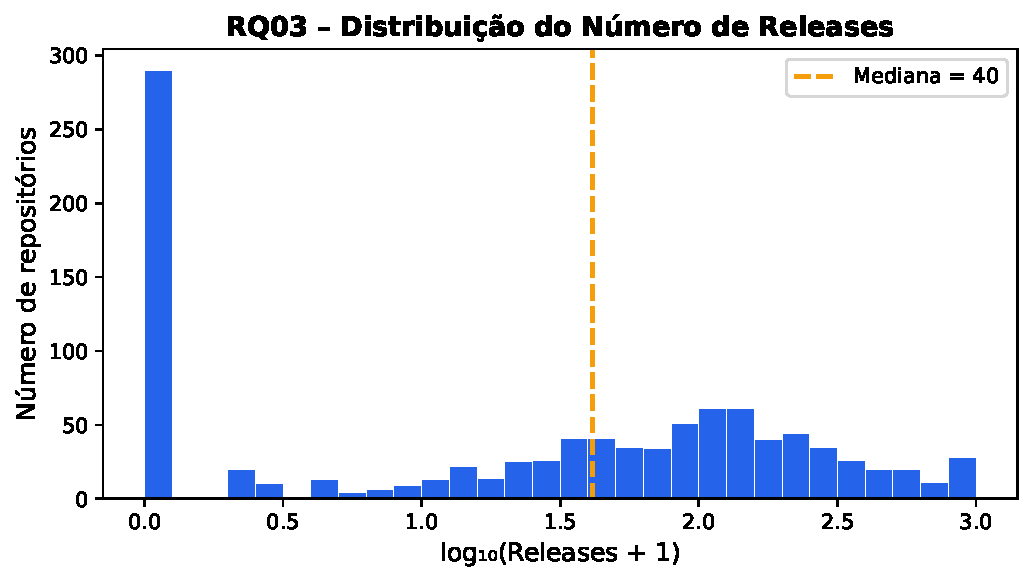
\includegraphics[width=0.85\textwidth]{figs/rq03_releases.pdf}
  \caption{Distribuição do número de releases (escala log\textsubscript{10}).}
  \label{fig:rq03}
\end{figure}

\textbf{Resultado:} a mediana é de \textbf{40 releases}.
Uma grande parcela dos repositórios possui zero ou poucas releases,
puxando a mediana para baixo.

\textbf{Discussão:} a hipótese H3 foi \textbf{confirmada em parte}.
Muitos projetos populares são repositórios de conteúdo (listas, documentação,
tutoriais) que não utilizam o mecanismo de releases do GitHub.
Projetos de software propriamente ditos tendem a ter muito mais releases.

% ──────────────────────────────────────────────────
\subsection{RQ04 -- Sistemas populares são atualizados com frequência?}
% ──────────────────────────────────────────────────

\textbf{Métrica:} número de dias desde a última atualização
(\texttt{days\_since\_update}).

\textbf{Hipótese (H4):} a maioria dos repositórios populares está atualizada
recentemente (últimos 30--60 dias).

\begin{figure}[H]
  \centering
  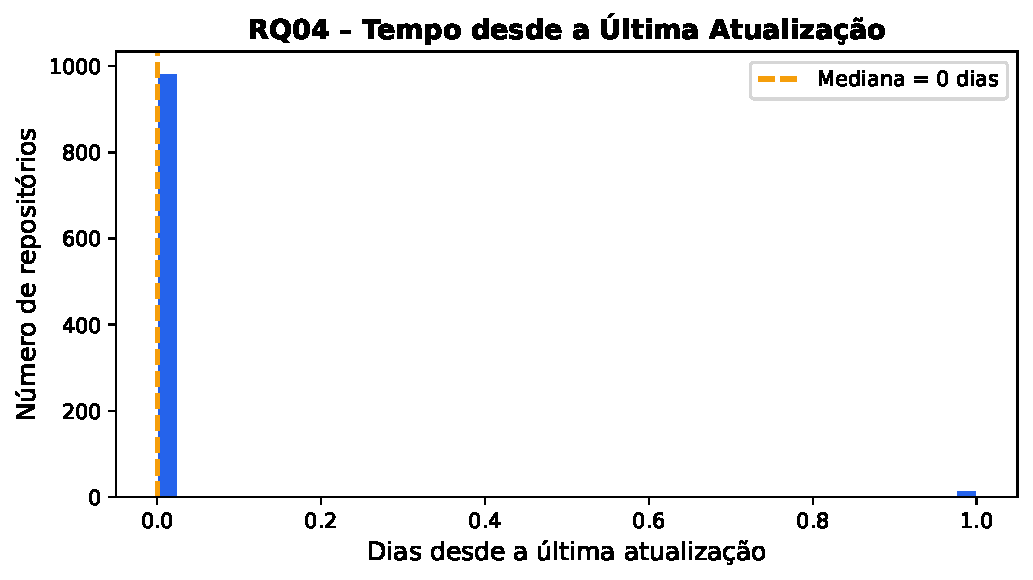
\includegraphics[width=0.85\textwidth]{figs/rq04_update.pdf}
  \caption{Distribuição do tempo desde a última atualização (dias).}
  \label{fig:rq04}
\end{figure}

\textbf{Resultado:} a mediana é de \textbf{0 dia(s)} desde a
última atualização. A concentração próxima de zero indica que a esmagadora
maioria dos repositórios populares foi atualizada muito recentemente
(na data de coleta, 6 de março de 2026).

\textbf{Discussão:} a hipótese H4 foi \textbf{fortemente confirmada}.
Repositórios populares são quase todos ativos e atualizados recentemente.

% ──────────────────────────────────────────────────
\subsection{RQ05 -- Sistemas populares são escritos nas linguagens mais populares?}
% ──────────────────────────────────────────────────

\textbf{Métrica:} linguagem primária de cada repositório.

\textbf{Hipótese (H5):} linguagens populares na comunidade open-source
(JavaScript/TypeScript, Python e Java) dominam os repositórios mais estrelados.

\begin{figure}[H]
  \centering
  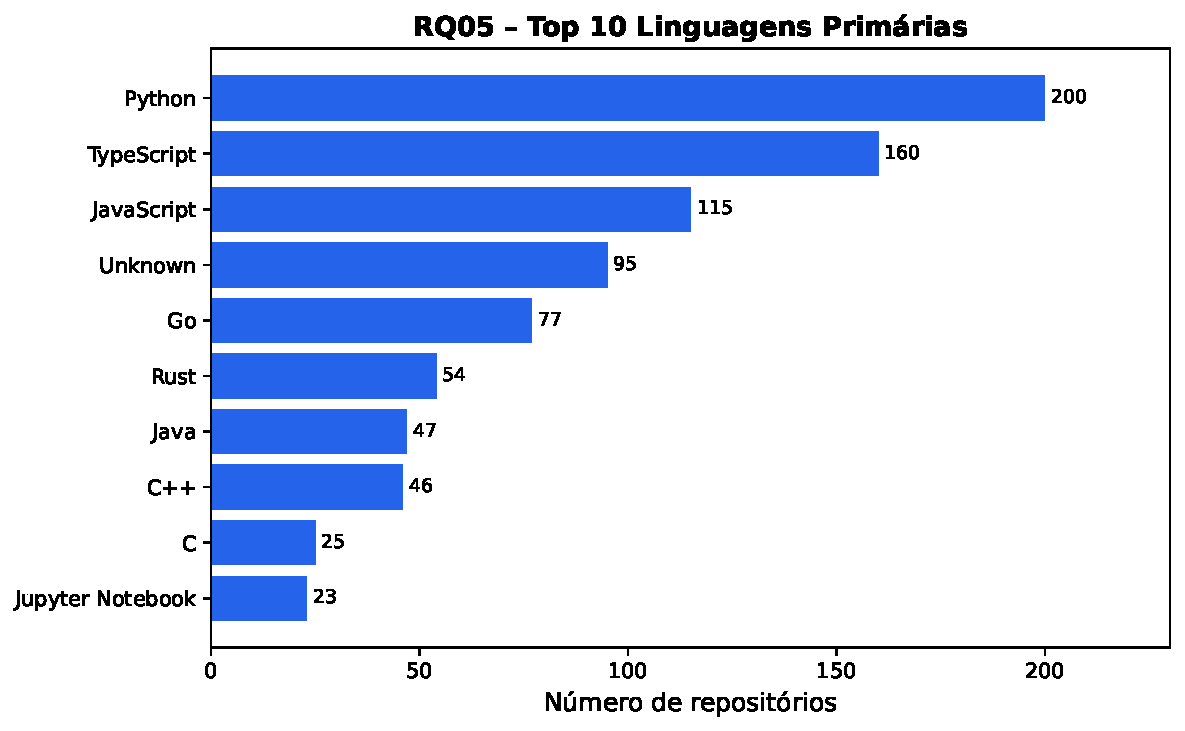
\includegraphics[width=0.85\textwidth]{figs/rq05_langs.pdf}
  \caption{Top 10 linguagens primárias nos 1.000 repositórios mais populares.}
  \label{fig:rq05}
\end{figure}

\begin{table}[H]
  \centering
  \caption{Top 10 linguagens primárias.}
  \label{tab:rq05}
  \begin{tabular}{lrr}
    \toprule
    \textbf{Linguagem} & \textbf{Repositórios} & \textbf{(\%)} \\
    \midrule
        Python & 200 & 20.0\% \\
        TypeScript & 160 & 16.0\% \\
        JavaScript & 115 & 11.5\% \\
        Unknown & 95 & 9.5\% \\
        Go & 77 & 7.7\% \\
        Rust & 54 & 5.4\% \\
        Java & 47 & 4.7\% \\
        C++ & 46 & 4.6\% \\
        C & 25 & 2.5\% \\
        Jupyter Notebook & 23 & 2.3\% \\
    \bottomrule
  \end{tabular}
\end{table}

\textbf{Resultado:} as linguagens que mais aparecem são
\textbf{Python (20,0\%), TypeScript (16,0\%), JavaScript (11,5\%)}, confirmando sua popularidade global.
A categoria ``Unknown'' representa repositórios sem linguagem de código
(documentação, listas, etc.).

\textbf{Discussão:} a hipótese H5 foi \textbf{confirmada}.
JavaScript/TypeScript e Python dominam o ecossistema open-source popular.

% ──────────────────────────────────────────────────
\subsection{RQ06 -- Sistemas populares possuem alto percentual de issues fechadas?}
% ──────────────────────────────────────────────────

\textbf{Métrica:} razão entre issues fechadas e total de issues
($\text{ratio} = \text{closed} / \text{total}$).

\textbf{Hipótese (H6):} projetos populares têm alto percentual de issues
fechadas (acima de 0,8), indicando manutenção ativa.

\begin{figure}[H]
  \centering
  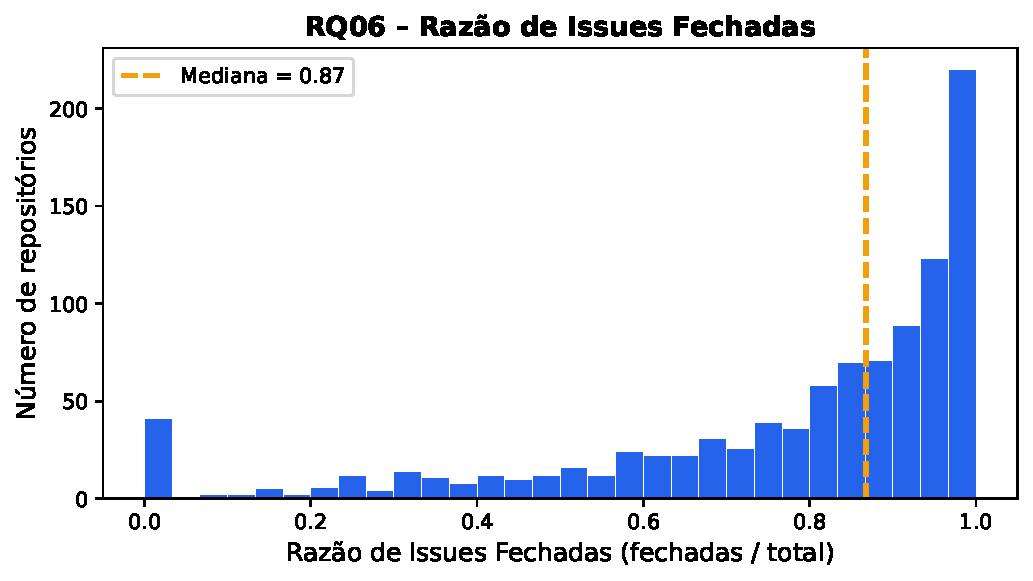
\includegraphics[width=0.85\textwidth]{figs/rq06_issues.pdf}
  \caption{Distribuição da razão de issues fechadas.}
  \label{fig:rq06}
\end{figure}

\textbf{Resultado:} a mediana da razão é de \textbf{0,8676},
ou seja, aproximadamente 86,76\% das issues são fechadas
nos repositórios medianos da amostra.

\textbf{Discussão:} a hipótese H6 foi \textbf{confirmada}.
A alta mediana indica que projetos populares são bem mantidos e que suas
equipes são responsivas no tratamento de issues.

% ─────────────────────────────────────────────────────────────────────────────
\subsection{RQ07 (Bônus) -- Linguagem e Contribuição Externa, Releases e Atualização}
% ─────────────────────────────────────────────────────────────────────────────

Esta questão de pesquisa bônus investiga se a linguagem primária do repositório
influencia as métricas das RQs 02, 03 e 04.

\textbf{Hipótese (H7):} linguagens mais populares tendem a receber mais
contribuições, lançar mais releases e manter atualizações mais frequentes.

\subsection{RQ07a -- PRs aceitas por linguagem}

\begin{figure}[H]
  \centering
  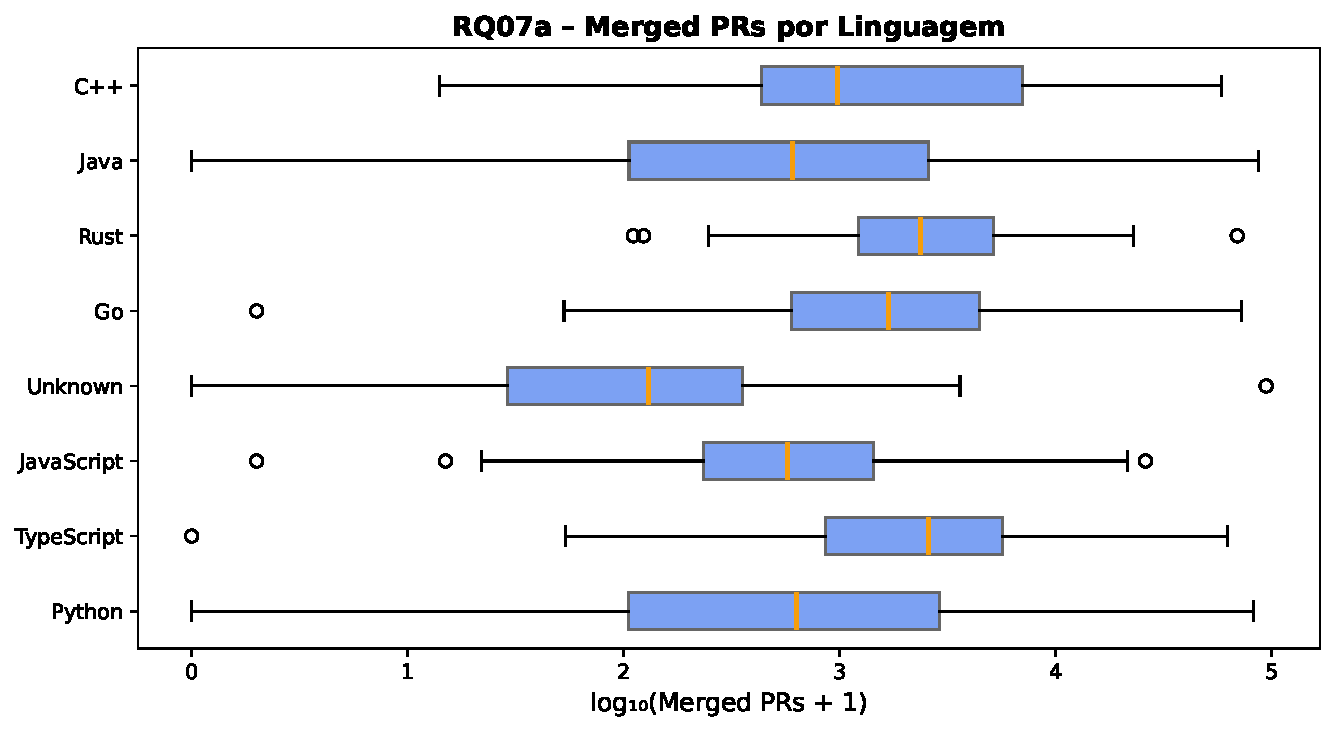
\includegraphics[width=0.85\textwidth]{figs/rq07a_prs_lang.pdf}
  \caption{Distribuição de PRs aceitas por linguagem (escala log\textsubscript{10}).}
  \label{fig:rq07a}
\end{figure}

\subsection{RQ07b -- Releases por linguagem}

\begin{figure}[H]
  \centering
  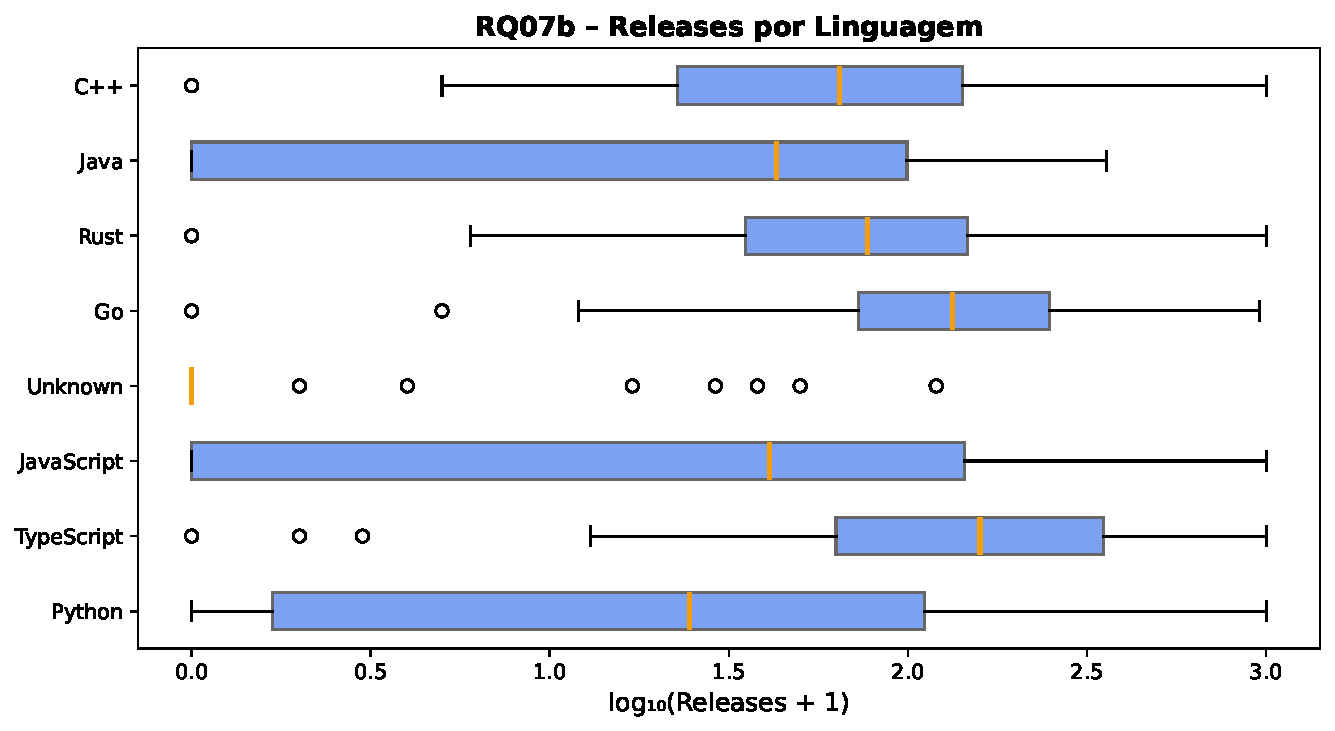
\includegraphics[width=0.85\textwidth]{figs/rq07b_releases_lang.pdf}
  \caption{Distribuição de releases por linguagem (escala log\textsubscript{10}).}
  \label{fig:rq07b}
\end{figure}

\subsection{RQ07c -- Tempo desde última atualização por linguagem}

\begin{figure}[H]
  \centering
  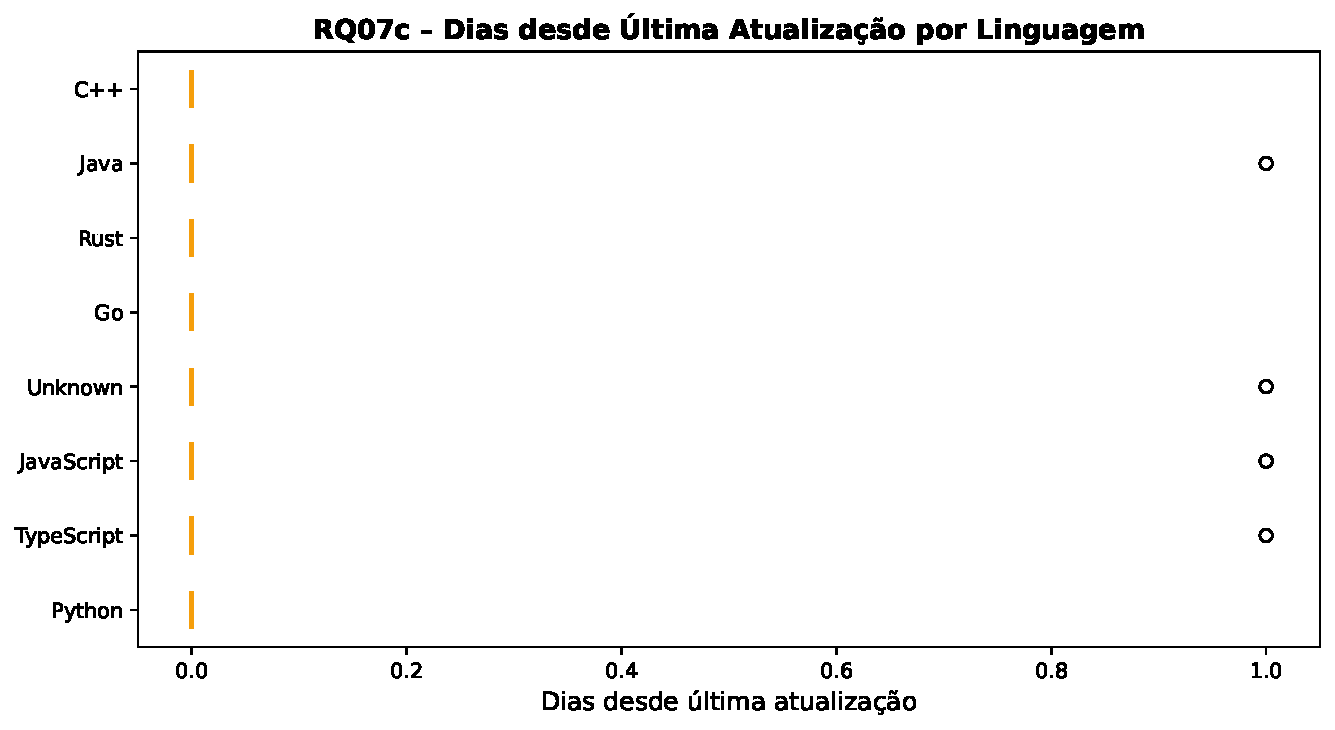
\includegraphics[width=0.85\textwidth]{figs/rq07c_update_lang.pdf}
  \caption{Distribuição de dias desde última atualização por linguagem.}
  \label{fig:rq07c}
\end{figure}

\begin{table}[H]
  \centering
  \caption{Medianas das métricas das RQs 02, 03 e 04 por linguagem (top 8).}
  \label{tab:rq07}
  \begin{tabular}{lrrrr}
    \toprule
    \textbf{Linguagem} & \textbf{Repos} &
    \textbf{Med. PRs} & \textbf{Med. Releases} & \textbf{Med. Dias Upd.} \\
    \midrule
        Python & 200 & 631 & 23 & 0 \\
        TypeScript & 160 & 2.588 & 158 & 0 \\
        JavaScript & 115 & 576 & 40 & 0 \\
        Unknown & 95 & 129 & 0 & 0 \\
        Go & 77 & 1.690 & 132 & 0 \\
        Rust & 54 & 2.371 & 76 & 0 \\
        Java & 47 & 605 & 42 & 0 \\
        C++ & 46 & 982 & 63 & 0 \\
    \bottomrule
  \end{tabular}
\end{table}

\textbf{Discussão:} a hipótese H7 é \textbf{parcialmente confirmada}.
Linguagens tipicamente usadas em projetos de software ativos (TypeScript,
Python, JavaScript, C++) tendem a apresentar medianas de PRs e releases mais
altas do que linguagens usadas em projetos de documentação (Markdown,
HTML, ``Unknown''). Quanto à frequência de atualização, a diferença entre
linguagens é menor, pois projetos de documentação também costumam ser
atualizados com frequência.

% ─────────────────────────────────────────────────────────────────────────────
\section{Discussão dos Resultados e Insights}
% ─────────────────────────────────────────────────────────────────────────────

\subsection{Insights Principais}

\begin{itemize}
  \item \textbf{Maturidade e popularidade caminham juntas:} a mediana de idade
    (8,39 anos) reforça que relevância em GitHub tende a ser
    construída no longo prazo.

  \item \textbf{Atividade recente é decisiva:} com mediana de 0
    dia(s) desde a última atualização, os projetos populares mostram alta
    manutenção contínua.

  \item \textbf{Contribuição externa é heterogênea:} a mediana de
    745 PRs aceitas convive com grande dispersão entre projetos
    de software e repositórios de conteúdo.

  \item \textbf{Releases não são universais:} apesar de projetos maduros,
    a mediana de 40 releases indica presença relevante de
    repositórios que não usam versionamento formal no GitHub.

  \item \textbf{Ecossistema concentrado em poucas linguagens:} Python (20,0\%), TypeScript (16,0\%), JavaScript (11,5\%)
    concentram uma fração expressiva dos repositórios analisados.

  \item \textbf{Manutenção de issues é elevada:} razão mediana de
    0,8676 sugere boa responsividade na gestão de demandas.
\end{itemize}

\subsection{Implicações para Projetos de Software}

Os resultados sugerem priorizar governança de contribuição (fluxo de PRs,
revisão e integração), cadência de atualização contínua e transparência sobre
estratégia de releases. Projetos que combinam esses fatores tendem a sustentar
engajamento e visibilidade no longo prazo.

% ─────────────────────────────────────────────────────────────────────────────
\section{Conclusão, Tomadas de Decisão e Resposta às Hipóteses}
% ─────────────────────────────────────────────────────────────────────────────

A análise dos 1000 repositórios mais populares do GitHub revelou que:

\begin{itemize}
  \item Repositórios populares são, em geral, \textbf{maduros} (mediana de
    8,39 anos) e \textbf{recentemente atualizados}
    (mediana de 0 dia(s) desde o último \textit{push}).

  \item A contribuição externa é significativa em projetos de código, com
    mediana de 745 PRs aceitas, embora projetos de
    documentação reduzam essa mediana.

  \item O uso de releases é heterogêneo: muitos repositórios populares são de
    conteúdo e não utilizam releases formais (mediana de 40).

  \item JavaScript/TypeScript e Python dominam as linguagens dos projetos
    populares.

  \item A manutenção é alta, com mediana de razão de issues fechadas de
    0,8676.

  \item Linguagens de código tendem a apresentar mais contribuição externa e
    mais releases do que repositórios de documentação.
\end{itemize}

\subsection{Tomadas de Decisão}

Com base nas evidências, recomendamos: (i) manter política explícita de
triagem e fechamento de issues; (ii) publicar releases periódicas para projetos
de software quando aplicável; (iii) documentar fluxo de contribuição para
absorver PRs externas; e (iv) monitorar recência de atualização como indicador
de saúde do projeto.

\subsection{Respondendo às Hipóteses (H1--H7)}

\begin{table}[H]
  \centering
  \caption{Síntese de confirmação das hipóteses.}
  \label{tab:hipoteses}
  \begin{tabular}{lp{8.5cm}l}
    Hipótese & Descrição resumida & Status \\
    \midrule
    H1 & Repositórios populares tendem a ser maduros. & Confirmada \\
    H2 & Projetos populares recebem muita contribuição externa. & Parcialmente confirmada \\
    H3 & Projetos populares lançam releases com frequência. & Parcialmente confirmada \\
    H4 & Projetos populares são atualizados com frequência. & Confirmada \\
    H5 & Linguagens populares dominam repositórios populares. & Confirmada \\
    H6 & Projetos populares têm alta razão de issues fechadas. & Confirmada \\
    H7 & Linguagem influencia contribuição, releases e atualização. & Parcialmente confirmada \\
    \bottomrule
  \end{tabular}
\end{table}

% ─────────────────────────────────────────────────────────────────────────────
\end{document}
